\documentclass[a4paper,12pt]{article}
\usepackage[utf8]{inputenc} % Required for inputting international characters
\usepackage[T1]{fontenc} % Output font encoding for international characters
\usepackage{float}
\usepackage{mathpazo} % Use the Palatino font by default
\usepackage[autostyle=true]{csquotes} % Required to generate language-dependent quotes in the bibliography
\usepackage{pdfpages}
\usepackage{amsmath}
\usepackage{subcaption}
\usepackage{xcolor}
\usepackage[square,numbers,sort]{natbib}
\usepackage{multirow}
\usepackage[newfloat]{minted} % Code listings, with syntax highlighting
\usepackage{caption}
\usepackage{tablefootnote} % for table footnotes
\usepackage{hyperref}
\usepackage[english]{babel}
\usepackage[useregional]{datetime2}
\usepackage[
    left = \flqq{},% 
    right = \frqq{},% 
    leftsub = \flq{},% 
    rightsub = \frq{} %
]{dirtytalk}
\usepackage{geometry}
\geometry{
	paper=a4paper, % Change to letterpaper for US letter
	inner=2.75cm, % Inner margin
	outer=3.5cm, % Outer margin
	bindingoffset=.5cm, % Binding offset
	top=2.5cm, % Top margin
	bottom=2.5cm, % Bottom margin
	%showframe, % Uncomment to show how the type block is set on the page
}
\usepackage{enumitem}
\usepackage{fdsymbol}
\usepackage{latexsym}
\usepackage{pdflscape}

\bibliographystyle{unsrtnat}

\newenvironment{code}{\captionsetup{type=listing}}{}
\SetupFloatingEnvironment{listing}{name=Código}

\hypersetup{
    colorlinks,
    linkcolor={red!80},
    citecolor={red!80},
    urlcolor={red!80}
}

\begin{document}

\pagenumbering{gobble} % remove page numbers (and reset to 1)

\newlist{dig}{itemize}{6}
\setlistdepth{6} 

% Configure the behaviour of levels entries
\setlist[dig, 1]
{label=$\medblacktriangleright$ , 
leftmargin=\parindent,
rightmargin=10pt
}
\setlist[dig, 2]
{label=$\smallblacktriangleright$, 
leftmargin=15pt,
rightmargin=15pt
}
\setlist[dig, 3]
{label=$\medtriangleright$, 
leftmargin=20pt,
rightmargin=20pt
}
\setlist[dig, 4]
{label=$\smalltriangleright$, 
leftmargin=25pt,
rightmargin=25pt
}
\setlist[dig, 5]
{label=$\Rightarrow$, 
leftmargin=30pt,
rightmargin=30pt
}
\setlist[dig, 6]
{label=$\rightarrow$, 
leftmargin=35pt,
rightmargin=25pt
}

% -------------------------------- Front page

\newcommand{\gh}{\href{https://github.com/Unike267}{gh:Unike267}}
\newcommand{\type}{Doctoral Programme in Engineering Physics}
\newcommand{\titulo}{Initial Research of the Thesis} % CHANGE HERE
\title{Title}
\newcommand{\subtitle}{\textit{\href{https://github.com/Unike267/Thesis}{gh:Unike267/Thesis}}}

% -------------------------------- Front content
\begin{center}\leavevmode
    \normalfont
    \includegraphics[width=1.05 \columnwidth]{figures/logos_perte.png}
    \vskip 10mm 
    \textit{\Large \gh}\\[1 cm]
    {\large \type}
    \vskip 5mm
    \rule{\linewidth}{0.2 mm}
    {\huge \bfseries \titulo \par}
    \vskip 5mm
    {\Large \bfseries \subtitle \par}
    \rule{\linewidth}{0.2 mm}\\[1.5 cm]
    \large
	\emph{\textbf{Author:}}\\
    Unai Sainz-Estebanez (Unike267)
    \vskip 5mm
	\emph{\textbf{ORCID:}}\\
    \href{https://orcid.org/0000-0002-4120-8313}{0000-0002-4120-8313}
    \vskip 20mm 
    \includegraphics[width=0.75 \columnwidth]{figures/logo.png}
    \vfill
    {\normalsize \today \par}
\end{center}
\cleardoublepage

\tableofcontents
\newpage
%\listoffigures
%\newpage
%\listoftables
%\newpage
%\listofalgorithms % List of algorithms in pseudocode format
%\newpage
%\listoflistings % List of algorithms in code format
%\newpage

\pagenumbering{arabic} % Arabic page numbers (and reset to 1)

% Sections
\section{Introduction}

\label{intro}

To start on this long way we will focus on the principal key words of this Thesis.

\vspace{5 mm}

\noindent These are: 

\begin{itemize}
\item Spiking Neural Networks
\item SPAD sensors
\item DVS sensors
\item TSN
\item RISC-V.
\end{itemize}

\subsection{Spiking Neural Networks}

\subsection{SPAD sensors}

SPAD (Single-Photon Avalanche Diode) \cite{9031298} sensors are an advanced type of photodiode sensor, specifically designed to detect extremely low amounts of light, to the single photon level. 
This makes them ideal for applications requiring exceptional sensitivity and the ability to measure extremely \textbf{fast} light events.

\vspace{5 mm}

\noindent Characteristics and Operation of SPADs:

\begin{itemize}
\item High Sensitivity
    \begin{itemize}
    \item[*] SPAD sensors can detect single photons, thanks to their ability to produce an \say{avalanche} of current when a single photon is detected.
    \item[*] This mechanism allows the sensor to significantly amplify the photon signal, providing a clear and strong response.
    \end{itemize}
\item Fast Response Time
    \begin{itemize}
    \item[*] SPADs are capable of recording events in times on the order of picoseconds.
    \item[*] This is useful in applications that require accurate photon arrival time (known as Time-of-Flight or TOF) measurements, such as in LIDAR and Time-Correlated Single Photon Counting (TCSPC), which is used in fluorescence studies.
    \end{itemize}
\item Geiger Mode Operation
    \begin{itemize}
    \item[*] SPADs operate in \say{Geiger} mode, which means that they are polarized at a voltage above the breakdown voltage. 
    \item[*] This causes an electron avalanche when a photon is detected, which allows the detection of the photon to be clearly recorded.
    \item[*] After detection, the sensor \textbf{needs a reset} to be ready for the next event.
    \end{itemize}
\item Dark noise/dark count noise
    \begin{itemize}
    \item[*] Although SPADs are very sensitive, they can suffer from “dark noise”, i.e. false signals caused by thermal electrons in the absence of light. 
    \item[*] This can be significantly controlled with cooling systems or by using signal processing techniques to filter out false events.
    \end{itemize}
\end{itemize}

\subsection{DVS sensors}

\subsection{TSN}

\subsection{RISC-V}



\newpage
\section{White Rabbit Node}
\label{wrn}

See White Rabbit Wiki \cite{WR:wiki}.

\begin{figure}[H]
    \centering
    \includegraphics[width=15cm]{figures/WR_node.pdf}
    \caption{WR Node.}
    \label{fig:WR-NODE}
\end{figure}

\newpage
\section{White Rabbit PTP Core}

The WR PTP (Precision Time Protocol) Core (WRPC) \cite{WR-core:wiki} \cite{WR-core:manual} \cite{WRPC:ohwr}, figure \ref{fig:WRPC}, is an Ethernet MAC implementation capable of providing precise timing. 
It can be used for sending and receiving regular Ethernet frames between user-defined HDL modules and a physical medium. 
It also implements the White Rabbit protocol to provide sub-nanosecond time synchronization.

\vspace{5 mm}

\noindent The White Rabbit PTP Core can operate in one of the following modes:
 
\begin{itemize}
\item GrandMaster:
    \begin{itemize}
    \item[>] WR Master synchronized to an external 1-PPS and 10 MHz clock signal, propagates precise timing to other WR-compliant devices.
    \end{itemize}
\item Master:
    \begin{itemize}
    \item[>] WR Master with free-running oscillator, propagates precise timing to other WR-compliant devices.
    \end{itemize}
\item Slave:
    \begin{itemize}
    \item[>] synchronizes its internal oscillator to another WR Master device.
    \end{itemize}
\end{itemize}

\begin{figure}[H]
    \centering
    \includegraphics[width=15cm]{figures/WRPC.pdf}
    \caption{WR PTP (Precision Time Protocol) Core (WRPC).}
    \label{fig:WRPC}
\end{figure}

\noindent You can find the HDL description of the WRPC internal components in \cite{WRPC:modules}.

\subsection{\textmu RV}

The \textmu RV \cite{urv-core:ohwr} \cite{urv-core:wiki} \cite{Włostowski:2213516} (Micro RISC-V) core is a small-sized implementation of a 32-bit RISC-V core, targeted specifically at FPGAs developed by CERN. 

\begin{figure}[H]
    \centering
    \includegraphics[width=5cm]{figures/urv_logo.png}
    \caption{\textmu RV logo.}
    \label{fig:urv}
\end{figure}

\begin{itemize}
\item Features:
    \begin{itemize}
    \item[>] Supports RV32IM instruction set. 
Division and multiply high instructions are optional and can be emulated to lower the FPGA footprint.
    \item[>] Target: FPGAs.
    \item[>] 4-stage pipeline (FDXW).
    \item[>] All instructions except taken branches/division in one clock cycle.
    \item[>] Code execution from internal memory block.
    \item[>] Wishbone bus (version B.4) for peripheral access.
    \item[>] Simple interrupt handling.
    \item[>] Verilog RTL code.
    \end{itemize}
\end{itemize}

\noindent Since \textmu RV is described in verilog and most of the WRPC component is in VHDL, it will be necessary to use a \textbf{mixed simulator} supported by VUnit.
In this context, one of the best options is \say{QuestaSim}.

\vspace{5mm}

\noindent \href{https://github.com/umarcor}{Umarcor} is planning to develop a container, hosted on our server, for this purpose. 
(DONE - Questa container, with and without VUnit, available on the lab server.)

\vspace{5mm}

\noindent \textbf{Task:} Learn how to generate a testbench using both HDLs: VHDL and Verilog.
(Initial mixed simulation test DONE - Unfortunately questa is a proprietary software and our server image cannot be distributed, so this example cannot be shown on GitHub, it is only available in our private GitLab repository.)

\newpage
\section{ASIC}
\label{asic}

The goal of this thesis is to perform this ASIC:

\begin{figure}[H]
    \centering
    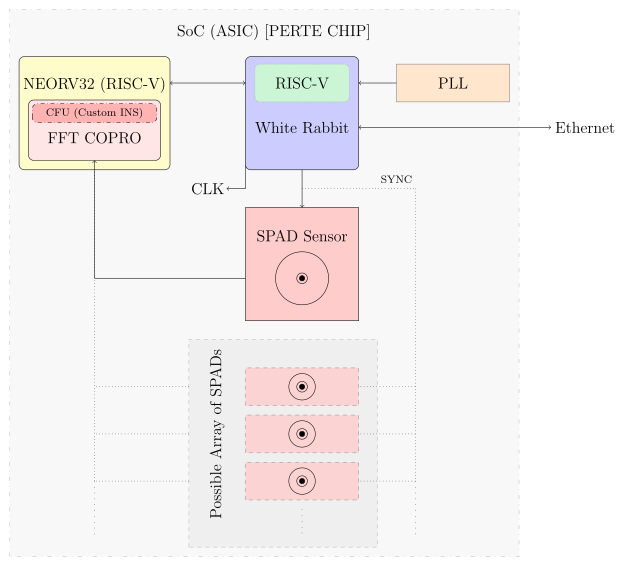
\includegraphics[width=14cm]{figures/ASIC-Scheme.pdf}
    \caption{ASIC to be develop.}
    \label{fig:ASIC}
\end{figure}

\newpage 
\section{Contributions}
\label{contrib}

\noindent The PhD student Unai Sainz Estebanez has made the following contributions to Open Hardware Repository \cite{ohwr}.

\vspace{5mm}

\noindent In the \href{https://gitlab.com/ohwr/project/urv-core}{urv-core} repository (December 19, 2024):

\begin{itemize}
\item Three commits:
    \begin{itemize}
    \item \href{https://gitlab.com/ohwr/project/urv-core/-/commit/655d46fe9fcb8a0880f63734f613a1f863b340ec}{655d46fe9fcb8a0880f63734f613a1f863b340ec}
    \item \href{https://gitlab.com/ohwr/project/urv-core/-/commit/d311497ac22b0164953fc0eb7474a97620c819e2}{d311497ac22b0164953fc0eb7474a97620c819e2}
    \item \href{https://gitlab.com/ohwr/project/urv-core/-/commit/46a6842f953cfab5f1814b8f09324b6f739e133f}{46a6842f953cfab5f1814b8f09324b6f739e133f}
    \end{itemize}
\end{itemize}

\noindent Related issue: \footnote{Since the migration from \say{ohwr.org} to \say{gitlab.com}, the authors of the issues created on the old site have been aliased by the person who performed the migration.}

\vspace{5mm}

\href{https://gitlab.com/ohwr/project/urv-core/-/issues/10}{gitlab.com/ohwr/project/urv-core/-/issues/10}

\vspace{5mm}

\noindent In the \href{https://gitlab.com/ohwr/project/general-cores/}{general-cores} repository (February 3, 2025):

\begin{itemize}
\item One commit:
    \begin{itemize}
    \item \href{https://gitlab.com/ohwr/project/general-cores/-/commit/4f887ca87620116b199a898599c70c69b0f0b5f0}{4f887ca87620116b199a898599c70c69b0f0b5f0}
    \end{itemize}
\end{itemize}

\noindent Related issue:

\vspace{5mm}

\href{https://gitlab.com/ohwr/project/general-cores/-/issues/57}{gitlab.com/ohwr/project/general-cores/-/issues/57}

\vspace{5mm}

\noindent In the \href{https://gitlab.com/ohwr/project/wr-cores/}{wr-cores} repository (February 13, 2025):

\begin{itemize}
\item One commit:
    \begin{itemize}
    \item \href{https://gitlab.com/ohwr/project/wr-cores/-/commit/c940635009eff0e417f9b547fbd73396f89e6627}{c940635009eff0e417f9b547fbd73396f89e6627}
    \end{itemize}
\end{itemize}

\noindent Related issue:

\vspace{5mm}

\href{https://gitlab.com/ohwr/project/wr-cores/-/issues/102}{gitlab.com/ohwr/project/wr-cores/-/issues/102}

\vspace{5mm}

\noindent In the \href{https://gitlab.com/ohwr/project/gn4124-core/}{gn4124-core} repository (February 14, 2025):

\begin{itemize}
\item Three commits:
    \begin{itemize}
    \item \href{https://gitlab.com/ohwr/project/gn4124-core/-/commit/eef550ec1e227704af35739ff2168e80eda70d75}{eef550ec1e227704af35739ff2168e80eda70d75}
    \item \href{https://gitlab.com/ohwr/project/gn4124-core/-/commit/b1fe3889dfffbf3f6b40f8a46886a659de09fbc7}{b1fe3889dfffbf3f6b40f8a46886a659de09fbc7}
    \item \href{https://gitlab.com/ohwr/project/gn4124-core/-/commit/71c4d362442ad11ddd2b1fd7fd4d8ab1e1947a89}{71c4d362442ad11ddd2b1fd7fd4d8ab1e1947a89}
    \end{itemize}
\end{itemize}

\noindent Related issue:

\vspace{5mm}

\href{https://gitlab.com/ohwr/project/wr-cores/-/issues/101}{gitlab.com/ohwr/project/wr-cores/-/issues/101}


\clearpage % If you want the references in a separate page
\bibliography{bibliography}

%\clearpage % If you want the appendix in a separate page
%\appendix
%\input{sections/appendix}

\end{document}
